%%%%%%%%%%%%%%%%
\section{Simulation Validation}
\label{sec:SimValidation}

GEANT4 is a toolkit implemented by the user so extensive efforts were completed in order to validate the results and ensure no bugs exists.
First steps were taken (for small runs) to compute the energy deposition for small runs by hand in order to make sure they agreeded with the analysis code.
In addition the reaction products of the \iso{Li}{6}$(\text{n},\alpha)$\iso{H}{3} were checked to make sure that they agreeded with the published values \footnote{GEANT4 4.9.2.p01 contains an error in which extra photons are generated, \verb+http://hypernews.slac.stanford.edu/HyperNews/geant4/get/phys-list/530.html+. This has been fixed in the release used, 4.9.5p1}.
The GEANT4 simulation was validated by comparing the single collision energy loss spectra in water and by comparing the simulation energy deposition to that of a measured spectra.


\subsection{Energy Deposition Validation}
The energy deposition was tested by reproducing the single collision energy loss spectra in water\footnote{%
An analysis class was not written for this simulation. 
Instead the verbosity of the simulation was set to \verb+verbose=1+ in the run macro.
The first ionisation collision (\verb+e-_G4DNAIonisation+) was then extracted with \verb+sed -n '/ParentID = 0/,/e-_G4DNAIonisation/p' G4OutputFileName.txt+ \verb+grep+ and \verb+awk+ were then used to extract the actual energy, \verb+| grep "e-\_G4DNAIonisatioin" | awk '${print $5}'+ %
}.
The \verb+PhysicsList+ was extended to include \verb+G4DNAPhysics+ and the detector material was set to the NIST definition contained in the toolkit with \verb+G4Material* H20 = man->FindOrBuildMaterial("G4_WATER")+.
In general there was excellent agreement between the simulated energy spectra and a previously published spectra\cite{turner_comparative_1982}.
The simulated spectra had much better resolution at fine energies (corresponding to discrete states) of which Turners did not.
%%%%%%%%%%%%%%%%%%%% Figures %%%%%%%%%%%%%%%%%%%%%%%%
\begin{figure}[h]
    \centering
    \begin{subfigure}[b]{0.45\figurewidth}
        \includegraphics[width=\textwidth]{SingleCollisionEnergyLoss_300bins}
        \caption{Simulated}
    \end{subfigure}
    \begin{subfigure}[b]{0.45\figurewidth}
        \includegraphics[width=\textwidth]{Turner_Fig2_SingleCollisionELoss}
        \caption{Single-collision energy loss spectra for electrons in water \protect\cite{turner_comparative_1982}}
        \caption{Published}
    \end{subfigure}
    \caption{Single Collision Energy Loss of Water}
\end{figure}
\subsection{Spectra Validation}
The simulated energy deposition is not the directly equivilant to light collected on the PMT because the scintillation process and light collection is not modeled.
However, the scintillation follows the energy deposition
The simulation was validated by computing the weighted average of the energy deposition \ref{eq:AvgEnergyDepDefination} and comparing it to the spectra average defined in \ref{eq:AvgChannelNumberDefination}.
%%%%%%%%%%%%%%%%%%%%% Equations %%%%%%%%%%%%%%%%%%%%%%
\begin{equation}
\label{eq:AvgEnergyDepDefination}
<E> = \frac{\int_0^\infty {\phi(E)EdE}}{\int_0^\infty{\phi(E)dE}} \\
\text{where}
\end{equation}
\begin{equation}
\label{eq:AvgChannelNumberDefination}
<\mu> = \frac{\int_0^\infty {f(x)xdx}}{\int_0^\infty{x(x)dx}} \\
\text{where}
\end{equation}
%%%%%%%%%%%%%%%%%%%% Figures %%%%%%%%%%%%%%%%%%%%%%%%
\begin{figure}
    \centering
    \caption{Gamma Simulation Agreement}
    \includegraphics[width=\textwidth]{G4EDep_LightYield_Co60}
    \label{fig:GammaSimAgreement}
\end{figure}
\begin{figure}
    \centering
    \caption{Neutron Simulation Agreement}
    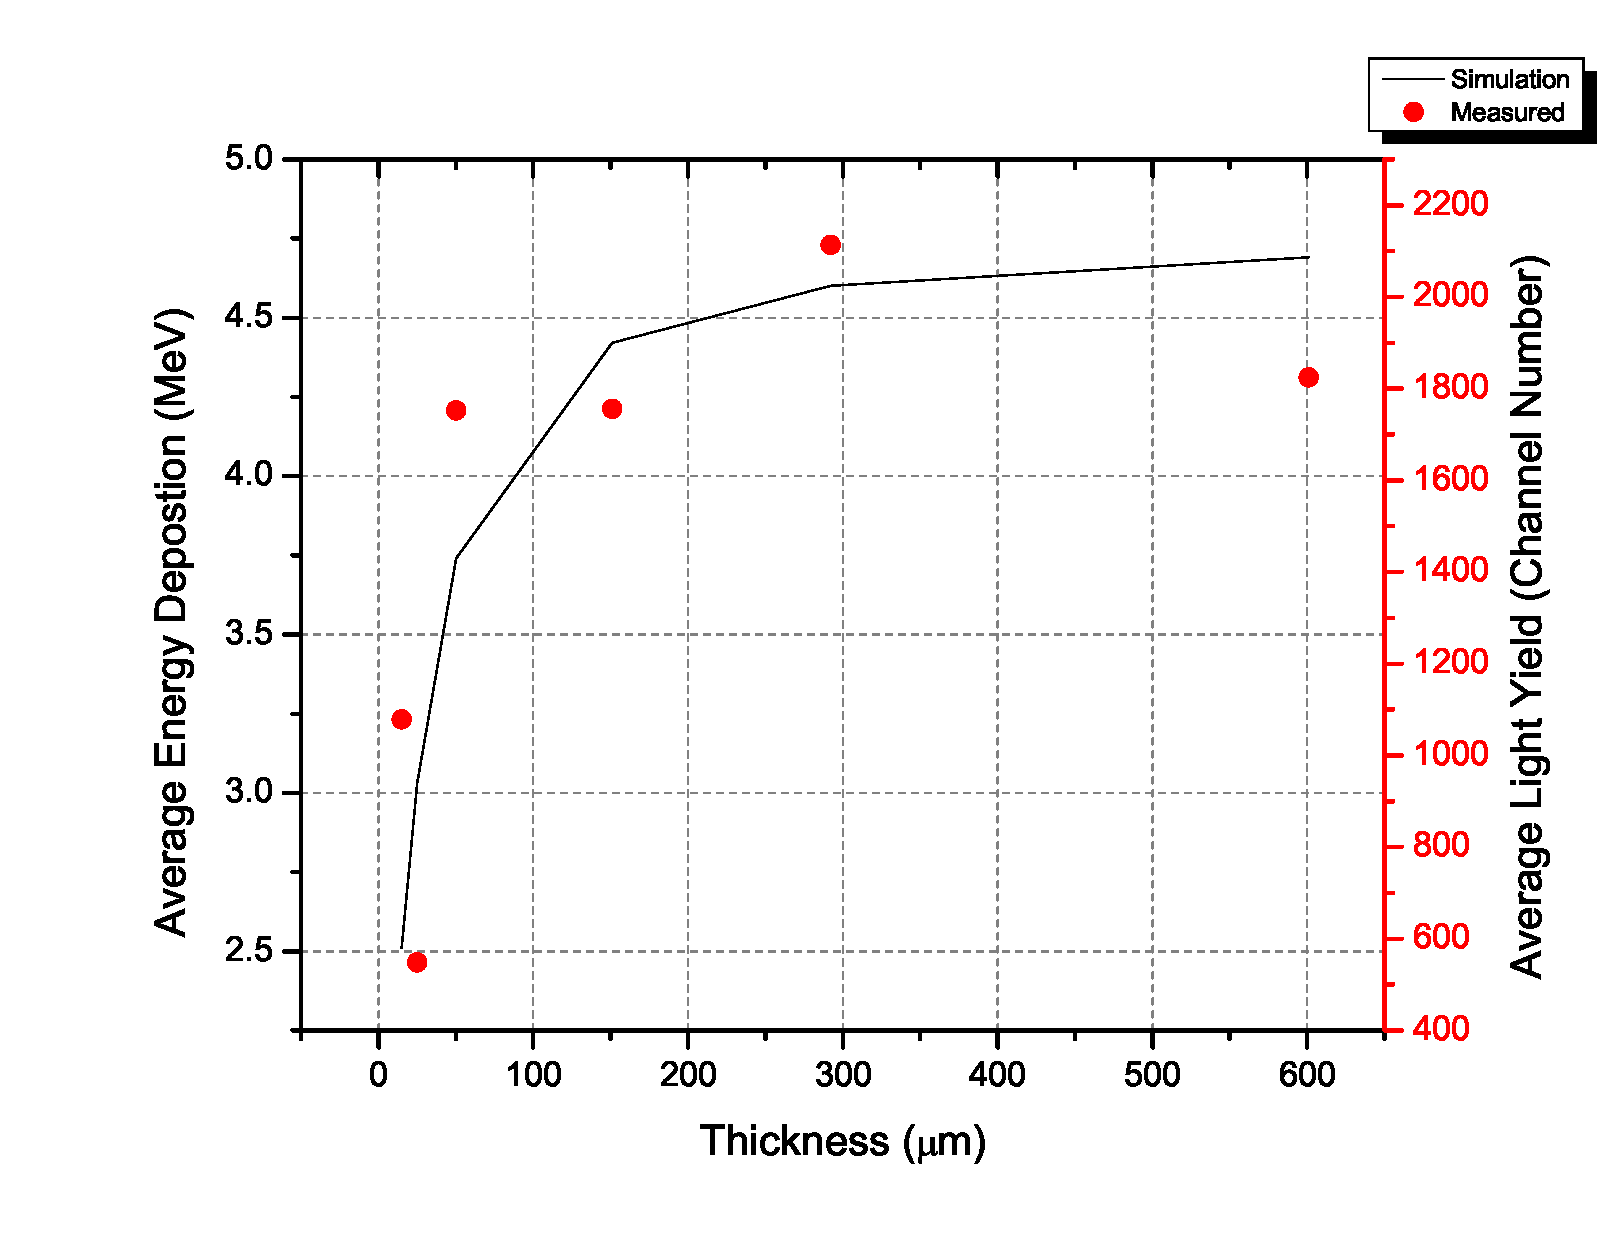
\includegraphics[width=\textwidth]{G4EDep_LightYield_Neutron}
    \label{fig:NeutronSimAgreement}
\end{figure}

